
\section{Estimating Probability Distributions: Neural Networks as Measure-Theoretic Estimators}

In the previous section, we showed how to avoid spurious correlation by modeling financial systems using \textbf{inclusion maps}, \textbf{vector clocks}, and \textbf{Lebesgue integration} over causality sets. We laid out a framework for identifying real causal structure—not just patterns that appear to be meaningful but dissolve under proper measure-theoretic scrutiny.

But we left something unresolved.

We talked about integrating over sets of causally significant events—like reactive trades, macroeconomic triggers, and their effects—but we never actually computed that integral. Why?

Because we don't know the integrand.

\textbf{There exists, in theory, some function that assigns ``causal weight'' to each event in the system.} A function that tells us how strongly a trade, a price movement, or a macro shock contributes to market behavior. But we can’t write it down explicitly. We know it exists—because the mathematics of measure theory and causality tells us it must—but it’s as elusive as the actual distribution behind a real-world coin flip.

What we need, then, is a way to \textit{discover} this function.

\subsection{Estimators: From Probability Theory to Machine Learning}

In classical statistics, this idea has a name: an \textbf{estimator}. An estimator is a function that guesses at some underlying ``true'' function based on observed data. It assumes the existence of a hidden structure—a real, ideal function—and seeks to approximate it as closely as possible.

Deep learning is just the modern, high-powered, measure-theoretic version of this idea.

You can think of it like a limiting process from calculus. In calculus, if we can define a function and a process for refining our guess (via derivatives, limits, etc.), we can get closer and closer to the true value. In deep learning, we do something similar—but instead of working in Euclidean space with distance metrics, we're working in \textbf{information space}, using tools from probability, entropy, and measure theory.

\subsection{Neural Networks as Universal Function Estimators}

Neural networks are powerful because they act as \textbf{universal function approximators}. That means: given enough data and capacity, they can learn to approximate \textit{any} function—including the elusive, abstract one that integrates causal weight over market event space.

In our case, that function isn't defined by simple math or clean formulas. It's defined over a \textbf{measurable space} \( (\Omega, \mathcal{F}, \mu) \), where each point represents a micro-event in the market—a trade, a price change, a news release. And the function we want to estimate is the one that maps these events to their causal impact.

What deep learning gives us is a principled way to approximate this function:

\[
\hat{f} \approx f^*, \quad \text{where } f^* \text{ is the true causal density function over } \Omega.
\]

The process is iterative—just like an \(\varepsilon\)--\(\delta\) proof in calculus. If we define our loss function correctly (analogous to an error bound), and we train on representative data, we can ensure that our approximation gets arbitrarily close to the real function within a certain tolerance.

\subsection{From Causal Geometry to Learning Geometry}

This moves us from the realm of hand-crafted mathematical models into a new regime: \textbf{causal learning}.

We're no longer trying to specify everything ourselves. We're acknowledging that the true structure exists in a high-dimensional, non-Euclidean, information-theoretic space—and we're building machines that can estimate it, refine it, and learn from it over time.

And just as calculus needed limits to define smooth motion, deep learning needs measure theory to define smooth inference. As long as our sets are well-defined and our data encodes meaningful events in the proper \(\sigma\)-algebra, we can develop estimators that converge to the ``true'' causal function—not just correlations that look good on paper.

\begin{quote}
\textit{Inclusion maps gave us the structure. Lebesgue integration gave us the calculus. Now neural networks give us the machinery to estimate what we couldn’t write down—and to do it in information space.}
\end{quote}



\subsubsection{How Neural Networks Estimate Causal Functions}

In the previous section, we noted that the true causal function \( f^* \colon \Omega \rightarrow \mathbb{R} \), which maps market events to their impact, exists within a high-dimensional, measure-theoretic space — but cannot be written down explicitly. What we can do, however, is build an \textit{estimator} that approximates it.

This is where neural networks come in.

A neural network is a parameterized function \( f_\theta(X) \), where \( \theta \) represents the trainable weights. Given data drawn from a measurable event space \( X \subset \Omega \), the network learns to approximate the unknown mapping:

\[
Y \approx f_\theta(X)
\]

Here, \( Y \) could represent anything from the probability of a price movement to the causal weight assigned to a trade, or the expected impact of a macroeconomic event. The key difference from classical models is that we do not assume a fixed structure like \( P(Y \mid X) \). Instead, the network learns this structure implicitly through training — using data sampled from the event space \( \Omega \), shaped by a measure \( \mu \).

In essence, we are not fitting a curve in Euclidean space — we are estimating a causal function in \textbf{information space}, using neural networks as high-capacity approximators under a measure-theoretic framework.

\subsubsection{Illustration: A Neural Estimator Over Market Events}

\begin{center}
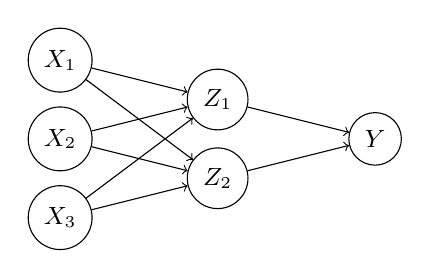
\begin{tikzpicture}[node distance=1.5cm, scale=1, every node/.style={scale=1}]
    % Input layer
    \node (x1) at (0,2) [draw, circle] {\small \(X_1\)};
    \node (x2) at (0,1) [draw, circle] {\small \(X_2\)};
    \node (x3) at (0,0) [draw, circle] {\small \(X_3\)};
    
    % Hidden layer
    \node (h1) at (2,1.5) [draw, circle] {\small \(Z_1\)};
    \node (h2) at (2,0.5) [draw, circle] {\small \(Z_2\)};
    
    % Output layer
    \node (y) at (4,1) [draw, circle] {\small \(Y\)};
    
    % Connections
    \foreach \i in {x1,x2,x3} {
        \foreach \j in {h1,h2} {
            \draw[->] (\i) -- (\j);
        }
    }
    \draw[->] (h1) -- (y);
    \draw[->] (h2) -- (y);
\end{tikzpicture}
\end{center}

\noindent In this simplified neural architecture:
\begin{itemize}
    \item Inputs \( X_1, X_2, X_3 \) might represent measurable features in our financial event space — such as trade size, volatility level, or recent price deltas.
    \item Hidden units \( Z_1, Z_2 \) capture intermediate structures — perhaps encoding temporal dependencies or interactions between causal sources.
    \item The output \( Y \) represents an estimated impact: for example, the expected future price change, or the inferred causal contribution of the event.
\end{itemize}

\textbf{Key Idea:} Instead of manually defining \( P(Y \mid X) \), we allow the network to learn a function that minimizes prediction error under a loss — effectively building a statistical estimator for the unknown causal mechanism.


\subsubsection{From Fixed Distributions to Adaptive Learning}

Up to this point, we've treated the causal function \( f^* \) as something that exists — hidden in the structure of the market — and neural networks as estimators that can approximate it. But there’s a deeper complication:

\begin{itemize}
    \item The function itself is not fixed.
    \item Financial markets are non-stationary: the distribution over events evolves as new information arrives.
    \item What appears causal in one regime (e.g., low volatility) may become irrelevant or even misleading in another (e.g., post-news shock).
\end{itemize}

In traditional models, we assume a static probability distribution — a fixed \( P(Y \mid X) \) — and hope it holds over time. But in high-frequency, data-rich environments, this assumption collapses. The true distribution is always shifting, always reacting — like the traders themselves.

\textbf{Therefore,} our estimators must not just approximate a fixed function — they must continuously \textit{adapt} to a changing measure space.

\vspace{0.5em}
Neural networks provide this adaptivity. Through online learning, gradient updates, or dynamic retraining, the parameterized function \( f_\theta \) evolves over time — effectively tracking a moving target within the larger measurable space \( (\Omega_t, \mathcal{F}_t, \mu_t) \). As new events reshape the space, the estimator learns to adjust:

\[
f_\theta^{(t+1)} \approx f^*_t \quad \text{for each new distribution } \mu_t.
\]

This turns the neural estimator into a kind of \textbf{information-theoretic compass} — constantly recalibrating itself to point toward the center of causal gravity, even as the terrain changes underneath.

\textit{But how do we ensure it adapts correctly?} That’s the question of convergence, generalization, and — crucially — how well we’ve defined the information geometry of the problem in the first place.


\subsection{Kullback-Leibler Divergence: Measuring Approximation Error in Information Space}

In the previous section, we framed neural networks as adaptive estimators operating over a shifting measure space. But even as these models update dynamically, there's a fundamental question we still need to answer:

\textbf{How close is our estimated function to the true causal structure?}

Mutual information helped us detect dependencies and isolate spurious correlations. But it doesn’t quantify the cost of approximation — the gap between what the model \textit{believes} and what the market actually \textit{does}.

This is where the \textbf{Kullback-Leibler (KL) divergence} enters the scene. It measures the information loss incurred when we replace a true distribution \( P \) with an estimated one \( Q \). In the context of deep learning, it tells us how far our learned distribution \( q(x) \) is from the underlying (and typically unknown) true distribution \( p(x) \):

\[
D_{KL}(P \,\|\, Q) = \int p(x) \log \frac{p(x)}{q(x)} \, d\mu(x).
\]

\vspace{0.5em}
Here:
\begin{itemize}
    \item \( p(x) \) is the true (but hidden) distribution of features or causal weights.
    \item \( q(x) \) is the model's current approximation — learned from data.
    \item \( d\mu(x) \) is the Lebesgue measure over the space \( \Omega \), ensuring the integration is valid across continuous event domains.
\end{itemize}

\textbf{KL divergence lives in information space.} It doesn't just measure numerical error — it quantifies epistemic drift: how much belief is lost when we trade ground truth for estimation.

As data flows through the layers of a neural network, the model refines its internal representations. But unless the KL divergence between the learned and true distributions shrinks over time, we're not converging — we're just reshaping our ignorance.

\vspace{0.5em}
\noindent
This gives us a concrete way to monitor learning as an information-theoretic process: not merely adjusting weights, but minimizing divergence in a high-dimensional probability landscape.

\begin{quote}
\textit{KL divergence is not just a loss function — it's a compass. It tells us how far our estimator has drifted from the truth in the topology of belief.}
\end{quote}

\subsubsection{Feature Selection in Decision Trees: A Discrete Case of Information Geometry}

To better understand how KL divergence operates in deep learning, it helps to first consider a simpler, discrete analogue — decision trees.

\paragraph{A Toy Model for Trade Decisions}

Imagine an automated trading system that uses a decision tree to determine whether to execute a trade based on observable features:

\begin{itemize}
    \item Trade Volume (\textbf{High} or \textbf{Low})
    \item Price Trend (\textbf{Up} or \textbf{Down})
\end{itemize}

The structure of the tree looks like this:

\begin{center}
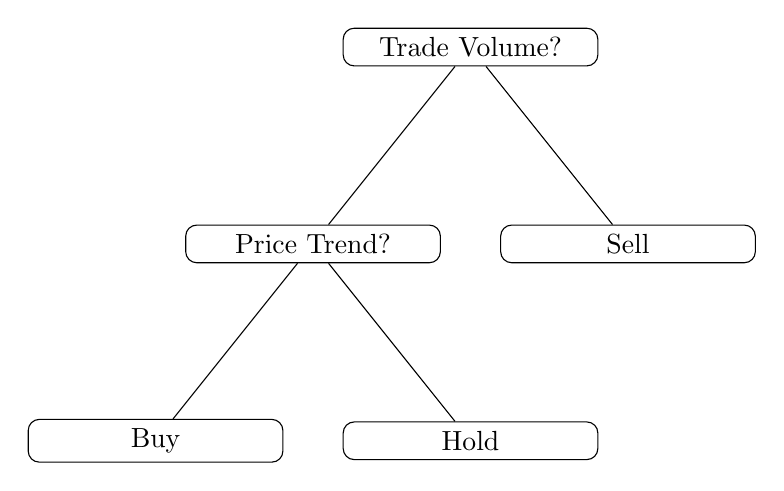
\begin{tikzpicture}[
    every node/.style={draw, rounded corners, text width=3cm, align=center},
    sibling distance=4cm,
    level distance=2.5cm
]
  % Root Node
  \node (root) {Trade Volume?}
    child { node (left) {Price Trend?}
        child { node (leftleft) {Buy} }
        child { node (leftright) {Hold} }
    }
    child { node (right) {Sell} };
\end{tikzpicture}
\end{center}

At each branching point, the tree selects the feature that maximally reduces uncertainty — measured using Shannon entropy:

\[
\text{Information Gain} = H(Y) - H(Y \mid X),
\]

where:
\begin{itemize}
    \item \( H(Y) \) is the entropy of trade outcomes before the split.
    \item \( H(Y \mid X) \) is the conditional entropy after splitting on feature \( X \).
\end{itemize}

This process is, in essence, a discrete optimization over information space. The tree is looking for directions that maximally collapse uncertainty — isolating features that carve the space into more certain regions.

\paragraph{From Trees to Tensors: Generalizing to Neural Networks}

While decision trees operate in discrete feature spaces, deep neural networks extend this idea to continuous, high-dimensional, and non-linear domains. But the core logic remains the same:

\begin{itemize}
    \item Identify patterns that reduce uncertainty.
    \item Choose representations that best approximate the true distribution.
    \item Minimize divergence from the structure of the data-generating process.
\end{itemize}

\textbf{In decision trees, this is called information gain. In neural networks, this is formalized as KL divergence.}

Instead of selecting a single feature at a node, neural networks \textit{learn a basis} of features across layers — continuously adjusting them to minimize information loss as data flows forward. KL divergence then serves as the information-theoretic counterpart to entropy-based feature selection: it quantifies how much "structure" is lost when the model’s internal representation diverges from the true causal geometry.

\vspace{1em}
\begin{quote}
\textit{Decision trees split to minimize entropy. Neural networks flow to minimize divergence. Both are just travelers in information space — trying to get closer to the truth.}
\end{quote}


\subsection{Variational Information Bottleneck: Structured Compression in Information Space}

So far, we’ve viewed KL divergence as a measure of information loss — a way to quantify how far our learned distribution diverges from the true causal structure. But in modern deep learning, KL divergence does more than diagnose approximation error.

\textbf{It becomes part of the optimization objective itself.}

In particular, \textbf{Variational Information Bottleneck (VIB)} methods use KL divergence to explicitly control what information the model retains — and what it throws away. The goal is no longer just to match the true distribution, but to compress irrelevant structure while preserving what matters for prediction.

The VIB principle formalizes this balance:

\[
\max I(X; Y) - \beta \, D_{KL}\big(P(Z \mid X) \,\|\, Q(Z)\big),
\]

where:
\begin{itemize}
    \item \( I(X; Y) \) is the mutual information between the input \( X \) and the output \( Y \) — i.e., how much predictive signal is retained.
    \item \( P(Z \mid X) \) is the encoder’s learned distribution over latent representations.
    \item \( Q(Z) \) is a simplified, low-information reference distribution (often standard normal).
    \item \( \beta \) is a tradeoff parameter controlling how much compression is enforced.
\end{itemize}

This objective encourages the model to represent only the \textit{minimal sufficient statistics} of \( X \) for predicting \( Y \). In measure-theoretic terms: it learns a transformation \( \phi: X \rightarrow Z \subset \Omega \) such that the image of \( X \) under \( \phi \) retains maximal causal structure, while discarding measure-zero noise.

\textbf{KL divergence acts like an information regularizer:} it penalizes complexity and forces the network to operate in a compressed, low-dimensional region of information space — one where causality survives and overfitting doesn’t.

\vspace{0.5em}
\noindent
This is the deep learning analogue of financial signal filtering. Just as a trading algorithm must discard random price jitters while acting on macroeconomic structure, VIB forces a model to throw away features that don’t carry predictive weight — no matter how tempting their local fluctuations may appear.

\begin{quote}
\textit{Inclusion maps isolated true structure. KL divergence measured how far we drifted. Now the information bottleneck tells us what to keep — and what to forget.}
\end{quote}





\begin{figure}[H]
\centering
\begin{tikzcd}[row sep=large, column sep=huge, ampersand replacement=\&]
{(X, P_X)} \arrow[r, "\phi", dashed] \arrow[dr, "f", swap] \& {(Z, P_Z)} \arrow[d, "\psi"] \\
\& {(Y, P_Y)}
\end{tikzcd}
\caption{A commutative diagram of the Variational Information Bottleneck. The encoder \( \phi \) maps inputs \( X \) to compressed representations \( Z \), discarding irrelevant information via KL divergence. The decoder \( \psi \) reconstructs predictions \( Y \), approximating the direct map \( f: X \rightarrow Y \).}
\end{figure}










\subsection{Visualizing Compression: Learning as a Commutative Flow}

To generalize the learning pattern we’ve described — from feature extraction to causal filtering — we can represent the process as a commutative diagram in information space. This isn’t just a schematic of network layers: it’s a diagram of inference through compression, where each transformation refines our understanding of the world.










\[
\begin{tikzpicture}[>=latex, scale=1.1, every node/.style={scale=1.2}]
  
  % Define matrix for the true feature distributions P(Z | X)
  \matrix (m) [matrix of math nodes, row sep=3.5em, column sep=7em] {
      X \\ 
      Z_1 \\ 
      Z_2 \\ 
      Z_3 \\ 
      P \\ % Final Prediction
  };

  % Define the simplified model Q(Z | X) to the right
  \matrix (q) [matrix of math nodes, row sep=3.5em, column sep=7em, right of=m, node distance=8cm] {
      \\  % No simplified version for X
      Q(Z_1 | X) \\ 
      Q(Z_2 | Z_1) \\ 
      Q(Z_3 | Z_2) \\ 
      Q(P | Z_3) \\ % Simplified Prediction
  };

  % Feature Transformations (Left Column)
  \path[->] (m-1-1) edge node[left] {$P(Z_1 | X)$} (m-2-1);
  \path[->] (m-2-1) edge node[left] {$P(Z_2 | Z_1)$} (m-3-1);
  \path[->] (m-3-1) edge node[left] {$P(Z_3 | Z_2)$} (m-4-1);
  \path[->] (m-4-1) edge node[left] {$P(P | Z_3)$} (m-5-1);

  % Simplified Feature Representations (Right Column)
  \path[->] (q-2-1) edge node[right] {$Q(Z_2 | Z_1)$} (q-3-1);
  \path[->] (q-3-1) edge node[right] {$Q(Z_3 | Z_2)$} (q-4-1);
  \path[->] (q-4-1) edge node[right] {$Q(P | Z_3)$} (q-5-1);

  % KL Divergence Regularization (Dashed Arrows)
  \path[->, dashed] (m-2-1.east) edge node[above] {$D_{KL}$} (q-2-1.west);
  \path[->, dashed] (m-3-1.east) edge node[above] {$D_{KL}$} (q-3-1.west);
  \path[->, dashed] (m-4-1.east) edge node[above] {$D_{KL}$} (q-4-1.west);
  \path[->, dashed] (m-5-1.east) edge node[above] {$D_{KL}(P(P \mid Z_3) \, \|\, Q(P \mid Z_3))$} (q-5-1.west);
  
\end{tikzpicture}
\]

At each stage, the model constructs two parallel representations:

\begin{itemize}
    \item On the left: the \textbf{true conditional distributions} — ideally aligned with the structure of the data-generating process.
    \item On the right: the \textbf{compressed approximations} — constrained, regularized, and filtered through KL divergence.
\end{itemize}

The model progresses layer by layer, mapping input \( X \) into latent variables \( Z_i \), and eventually into a prediction \( P \). At every point, KL divergence acts as a tension between expressivity and parsimony — enforcing structure while penalizing unnecessary complexity.



\vspace{1em}
This diagram illustrates what learning looks like under a measure-theoretic lens: a flow through nested spaces of reduced uncertainty. Each \( D_{KL} \) is a checkpoint — a formal request for the model to justify its complexity, to compress responsibly, and to make its structure match the data’s causality.

\begin{quote}
\textit{Learning isn’t just moving forward — it’s narrowing. Each layer carves away irrelevance. Each KL divergence asks: “Are you closer to the truth, or just louder?”}
\end{quote}

The commutative diagram we just introduced isn’t merely a technical schematic. It visually encodes the logic of inference under constraint — a flow of information from raw observations to structured predictions, filtered through a series of transformations that shape and prune the model’s internal geometry.

KL divergence serves as the gatekeeper between expressive power and epistemic discipline: it pressures the model to compress aggressively, but not blindly.

\subsubsection{Nodes as Layers in Information Space}

Each node in the diagram represents a distinct stage in the evolution of knowledge:

\begin{itemize}
    \item \textbf{\( X \) (Raw Inputs):} The measurable substrate — bid-ask spreads, order book velocity, trade volume — from which the model begins constructing a representation.
    
    \item \textbf{\( Z_1, Z_2, Z_3 \) (Latent Representations):} Intermediate encodings in the model's internal space, successively transformed and refined. Each layer restructures the measure on \( \Omega \), ideally concentrating information relevant for prediction while discarding noise.
    
    \item \textbf{\( P \) (Final Prediction):} A probability distribution over future events (e.g., price movements) — the model’s best estimate of downstream outcomes based on its internal representation.
    
    \item \textbf{\( Q(Z_i | \cdot) \) (Regularized Approximations):} Constrained, compressed versions of each latent feature — simpler distributions with lower entropy, used as references during training to prevent overfitting and encourage generalization.
\end{itemize}


\[
\resizebox{\textwidth}{!}{
\begin{tikzpicture}[>=latex, scale=1.1, every node/.style={scale=1.2}, node distance=2.2cm]

  % Define matrix of math nodes (just the symbols)
  \matrix (m) [matrix of math nodes, row sep=3.8em, column sep=10em] {
      X \\
      Z_1 \\
      Z_2 \\
      Z_3 \\
      P \\
  };

  \matrix (q) [matrix of math nodes, row sep=3.8em, column sep=10em, right of=m, node distance=7.5cm] {
      \\ % X has no simplified version
      Q(Z_1|X) \\
      Q(Z_2|Z_1) \\
      Q(Z_3|Z_2) \\
      Q(P|Z_3) \\
  };

  % Arrows (structure only)
  \path[->] (m-1-1) edge (m-2-1);
  \path[->] (m-2-1) edge (m-3-1);
  \path[->] (m-3-1) edge (m-4-1);
  \path[->] (m-4-1) edge (m-5-1);

  \path[->] (q-2-1) edge (q-3-1);
  \path[->] (q-3-1) edge (q-4-1);
  \path[->] (q-4-1) edge (q-5-1);

  \path[->, dashed] (m-2-1.east) edge (q-2-1.west);
  \path[->, dashed] (m-3-1.east) edge (q-3-1.west);
  \path[->, dashed] (m-4-1.east) edge (q-4-1.west);
  \path[->, dashed] (m-5-1.east) edge (q-5-1.west);

  % Left-side annotations (closer spacing)
  \node[left=0.2cm of m-1-1] {\parbox{4cm}{\raggedleft\footnotesize \textit{Raw Inputs}\\\textit{(e.g., order book, volume)}}};
  \node[left=0.2cm of m-2-1] {\parbox{4cm}{\raggedleft\footnotesize \textit{Latent Layer 1}\\\textit{(initial encoding)}}};
  \node[left=0.2cm of m-3-1] {\parbox{4cm}{\raggedleft\footnotesize \textit{Latent Layer 2}\\\textit{(refined representation)}}};
  \node[left=0.2cm of m-4-1] {\parbox{4cm}{\raggedleft\footnotesize \textit{Latent Layer 3}\\\textit{(prediction-ready signal)}}};
  \node[left=0.2cm of m-5-1] {\parbox{4cm}{\raggedleft\footnotesize \textit{Final Prediction}\\\textit{(distribution over outcomes)}}};

  % Right-side annotations (closer spacing)
  \node[right=0.2cm of q-2-1] {\parbox{4cm}{\raggedright\footnotesize \textit{Approx. of $Z_1$}\\\textit{(lower entropy)}}};
  \node[right=0.2cm of q-3-1] {\parbox{4cm}{\raggedright\footnotesize \textit{Approx. of $Z_2$}\\\textit{(regularized)}}};
  \node[right=0.2cm of q-4-1] {\parbox{4cm}{\raggedright\footnotesize \textit{Approx. of $Z_3$}\\\textit{(compressed)}}};
  \node[right=0.2cm of q-5-1] {\parbox{4cm}{\raggedright\footnotesize \textit{Approx. Prediction}\\\textit{(reference dist.)}}};

\end{tikzpicture}
}
\]

\subsubsection*{Qualitative Interpretations of Diagram Nodes}

\vspace{1em}
\textbf{Left-Side (Main Path) Explanations}

\begin{itemize}
    \item \textbf{Raw Inputs (e.g., order book, volume)}: This is the raw substrate — the measurable phenomena the model observes. Think timestamped price ticks, trade volumes, order book changes. This layer is closest to the physical world and contains high entropy: it’s rich, unfiltered, and noisy.

    \item \textbf{Latent Layer 1 (initial encoding)}: The model’s first attempt at structure. This is where raw signals are projected into a lower-dimensional space that begins to highlight patterns — perhaps short-term momentum, microstructure signals, or statistical anomalies. Still close to the input space, but with noise partially filtered out.

    \item \textbf{Latent Layer 2 (refined representation)}: The middle abstraction. By now, the model is combining multiple signals into more complex, abstract concepts — e.g., implicit volatility regimes, mean-reverting behaviors, or early indicators of liquidity shifts. The information has been compacted and made more relevant for the final task.

    \item \textbf{Latent Layer 3 (prediction-ready signal)}: This is the final bottleneck before decision-making. At this point, most of the irrelevant entropy has been discarded, and what remains is a high-fidelity encoding optimized for forecasting — a minimal but sufficient statistic, so to speak, for making predictions.

    \item \textbf{Final Prediction (distribution over outcomes)}: The model’s output is not a single number, but a distribution over possible futures — often expressed as class probabilities or conditional expectations. This represents the model’s internal belief, formed from compressed and transformed versions of the raw inputs.
\end{itemize}

\vspace{1em}
\textbf{Right-Side (Regularized Approximations) Explanations}

\begin{itemize}
    \item \textbf{Approximation of \( Z_1 \) (lower entropy)}: A simplified version of the initial encoding. This approximation strips out some complexity to prevent overfitting and helps guide the model to learn generalizable features. It’s like teaching with a textbook summary instead of an encyclopedia.

    \item \textbf{Approximation of \( Z_2 \) (regularized)}: A soft constraint on the second latent layer. The idea here is to keep the model from encoding too much nuance in the middle layers by anchoring them to distributions that reflect simpler or smoothed behavior — effectively acting as a form of structural prior.

    \item \textbf{Approximation of \( Z_3 \) (compressed)}: This approximation enforces parsimony just before the prediction head. By regularizing the penultimate layer, we force the model to make decisions using only what’s strictly necessary — leading to better generalization under distributional shift.

    \item \textbf{Approximate Prediction (reference distribution)}: A reference prediction used during training — often a softened, distilled, or averaged version of the true output distribution. This acts like a "teacher signal" to stabilize learning and align the model’s confidence with broader trends rather than local quirks.
\end{itemize}





\subsubsection{Solid Arrows: The Flow of Representation}

The vertical arrows on the left trace the model’s expressive path — how it builds increasingly abstract representations through conditional transformations:

\[
P(Z_1 \mid X), \quad P(Z_2 \mid Z_1), \quad P(Z_3 \mid Z_2), \quad P(P \mid Z_3).
\]

On the right, the vertical arrows represent a simplified model — one that passes through lower-dimensional or constrained approximations:

\[
Q(Z_2 \mid Z_1), \quad Q(Z_3 \mid Z_2), \quad Q(P \mid Z_3).
\]

\[
\resizebox{\textwidth}{!}{
\begin{tikzpicture}[>=latex, scale=1.1, every node/.style={scale=1.2}]

  % Define matrix for the true feature distributions P(Z | X)
  \matrix (m) [matrix of math nodes, row sep=3.5em, column sep=7em] {
      X \\ 
      Z_1 \\ 
      Z_2 \\ 
      Z_3 \\ 
      P \\ % Final Prediction
  };

  % Define the simplified model Q(Z | X) to the right
  \matrix (q) [matrix of math nodes, row sep=3.5em, column sep=7em, right of=m, node distance=8cm] {
      \\  % No simplified version for X
      Q(Z_1 | X) \\ 
      Q(Z_2 | Z_1) \\ 
      Q(Z_3 | Z_2) \\ 
      Q(P | Z_3) \\ % Simplified Prediction
  };

  % Feature Transformations (Left Column) with parbox annotations
  \path[->] (m-1-1) edge node[left=0.2cm] {\parbox{4cm}{\raggedleft\footnotesize \textit{Model builds abstraction}\\[-0.2em] $P(Z_1 \mid X)$}} (m-2-1);
  \path[->] (m-2-1) edge node[left=0.2cm] {\parbox{4cm}{\raggedleft\footnotesize \textit{Refines structure}\\[-0.2em] $P(Z_2 \mid Z_1)$}} (m-3-1);
  \path[->] (m-3-1) edge node[left=0.2cm] {\parbox{4cm}{\raggedleft\footnotesize \textit{Distills signal}\\[-0.2em] $P(Z_3 \mid Z_2)$}} (m-4-1);
  \path[->] (m-4-1) edge node[left=0.2cm] {\parbox{4cm}{\raggedleft\footnotesize \textit{Final forecast}\\[-0.2em] $P(P \mid Z_3)$}} (m-5-1);

  % Simplified Feature Representations (Right Column) with parbox annotations
  \path[->] (q-2-1) edge node[right=0.2cm] {\parbox{4cm}{\raggedright\footnotesize \textit{Simplified structure}\\[-0.2em] $Q(Z_2 \mid Z_1)$}} (q-3-1);
  \path[->] (q-3-1) edge node[right=0.2cm] {\parbox{4cm}{\raggedright\footnotesize \textit{Compressed signal}\\[-0.2em] $Q(Z_3 \mid Z_2)$}} (q-4-1);
  \path[->] (q-4-1) edge node[right=0.2cm] {\parbox{4cm}{\raggedright\footnotesize \textit{Baseline prediction}\\[-0.2em] $Q(P \mid Z_3)$}} (q-5-1);

  % KL Divergence Regularization (Dashed Arrows)
  \path[->, dashed] (m-2-1.east) edge node[above] {} (q-2-1.west);
  \path[->, dashed] (m-3-1.east) edge node[above] {} (q-3-1.west);
  \path[->, dashed] (m-4-1.east) edge node[above] {} (q-4-1.west);
  \path[->, dashed] (m-5-1.east) edge node[above] {} (q-5-1.west);

  % Phantom annotations for nodes (preserve spacing)
  \node[left=0.2cm of m-1-1] {\phantom{\parbox{4cm}{\raggedleft\footnotesize \textit{Raw Inputs}\\\textit{(e.g., order book, volume)}}}};
  \node[left=0.2cm of m-2-1] {\phantom{\parbox{4cm}{\raggedleft\footnotesize \textit{Latent Layer 1}\\\textit{(initial encoding)}}}};
  \node[left=0.2cm of m-3-1] {\phantom{\parbox{4cm}{\raggedleft\footnotesize \textit{Latent Layer 2}\\\textit{(refined representation)}}}};
  \node[left=0.2cm of m-4-1] {\phantom{\parbox{4cm}{\raggedleft\footnotesize \textit{Latent Layer 3}\\\textit{(prediction-ready signal)}}}};
  \node[left=0.2cm of m-5-1] {\phantom{\parbox{4cm}{\raggedleft\footnotesize \textit{Final Prediction}\\\textit{(distribution over outcomes)}}}};

  \node[right=0.2cm of q-2-1] {\phantom{\parbox{4cm}{\raggedright\footnotesize \textit{Approx. of $Z_1$}\\\textit{(lower entropy)}}}};
  \node[right=0.2cm of q-3-1] {\phantom{\parbox{4cm}{\raggedright\footnotesize \textit{Approx. of $Z_2$}\\\textit{(regularized)}}}};
  \node[right=0.2cm of q-4-1] {\phantom{\parbox{4cm}{\raggedright\footnotesize \textit{Approx. of $Z_3$}\\\textit{(compressed)}}}};
  \node[right=0.2cm of q-5-1] {\phantom{\parbox{4cm}{\raggedright\footnotesize \textit{Approx. Prediction}\\\textit{(reference dist.)}}}};

\end{tikzpicture}
}
\]

\subsubsection*{Qualitative Interpretations of Transformational Arrows}

\vspace{1em}
\textbf{Left Column (True Representation Path)}

\begin{itemize}
    \item \textbf{Model builds abstraction ($P(Z_1 \mid X)$)}\\
    The first transformation learns to represent the high-dimensional, noisy raw input \( X \) into a structured latent form \( Z_1 \). This step begins the process of abstraction: reducing dimensionality and identifying signal amidst the noise.

    \item \textbf{Refines structure ($P(Z_2 \mid Z_1)$)}\\
    The second layer takes the initial encoding and deepens the model’s understanding. Here, the representation is made more abstract and structured — capturing higher-order patterns, dependencies, or temporal dynamics in the data.

    \item \textbf{Distills signal ($P(Z_3 \mid Z_2)$)}\\
    The third layer strips the representation down to its essential predictive content. Non-essential variance is discarded, concentrating the signal into a form that is maximally informative for downstream prediction.

    \item \textbf{Final forecast ($P(P \mid Z_3)$)}\\
    The model uses the final latent representation to make its ultimate prediction. This step projects the abstract signal into a concrete probability distribution over future events — i.e., the model’s belief.
\end{itemize}

\vspace{1em}
\textbf{Right Column (Simplified Reference Path)}

\begin{itemize}
    \item \textbf{Simplified structure ($Q(Z_2 \mid Z_1)$)}\\
    A lower-complexity approximation of the second latent transformation. This version intentionally reduces detail and expressiveness — guiding the model to learn smoother, more generalizable features at the cost of some precision.

    \item \textbf{Compressed signal ($Q(Z_3 \mid Z_2)$)}\\
    A compact representation of the third latent layer, designed to act as a bottleneck. It encourages the model to express relevant information with fewer bits — enforcing parsimony and robustness to noise.

    \item \textbf{Baseline prediction ($Q(P \mid Z_3)$)}\\
    A simplified predictive distribution derived from the compressed latent. Often serves as a regularization target — anchoring the model's final prediction toward a conservative, low-variance baseline during training.
\end{itemize}



\subsubsection{Dashed Arrows: Divergence as a Compression Constraint}

The horizontal dashed arrows represent the core regulatory mechanism of this system:

\[
D_{KL}\big(P(Z_i \mid \cdot) \, \| \, Q(Z_i \mid \cdot)\big),
\]

which measure how far the expressive model has deviated from its compressed baseline. These divergences are not errors — they are costs. And the model pays them only when the information gained is worth the entropy spent.

Each KL divergence acts like a tax on complexity. The model must “justify” every bit of additional structure by proving that it contributes to the predictive integrity of the system. Otherwise, the regularized approximation pulls the model back toward simplicity.

\begin{quote}
\textit{What emerges is a balance: expressive enough to model causality, but compressed enough to generalize. Each layer doesn't just learn — it negotiates.}
\end{quote}



\[
\resizebox{\textwidth}{!}{
\begin{tikzpicture}[>=latex, scale=1.1, every node/.style={scale=1.2}]

  % Define matrix for the true feature distributions P(Z | X)
  \matrix (m) [matrix of math nodes, row sep=3.5em, column sep=7em] {
      X \\ 
      Z_1 \\ 
      Z_2 \\ 
      Z_3 \\ 
      P \\ % Final Prediction
  };

  % Define the simplified model Q(Z | X) to the right
  \matrix (q) [matrix of math nodes, row sep=3.5em, column sep=7em, right of=m, node distance=8cm] {
      \\  % No simplified version for X
      Q(Z_1 | X) \\ 
      Q(Z_2 | Z_1) \\ 
      Q(Z_3 | Z_2) \\ 
      Q(P | Z_3) \\ % Simplified Prediction
  };

  % Feature Transformations (Left Column) — now phantom
  \path[->] (m-1-1) edge node[left=0.2cm] {\phantom{\parbox{4cm}{\raggedleft\footnotesize \textit{Model builds abstraction}\\[-0.2em] $P(Z_1 \mid X)$}}} (m-2-1);
  \path[->] (m-2-1) edge node[left=0.2cm] {\phantom{\parbox{4cm}{\raggedleft\footnotesize \textit{Refines structure}\\[-0.2em] $P(Z_2 \mid Z_1)$}}} (m-3-1);
  \path[->] (m-3-1) edge node[left=0.2cm] {\phantom{\parbox{4cm}{\raggedleft\footnotesize \textit{Distills signal}\\[-0.2em] $P(Z_3 \mid Z_2)$}}} (m-4-1);
  \path[->] (m-4-1) edge node[left=0.2cm] {\phantom{\parbox{4cm}{\raggedleft\footnotesize \textit{Final forecast}\\[-0.2em] $P(P \mid Z_3)$}}} (m-5-1);

  % Simplified Feature Representations (Right Column) — now phantom
  \path[->] (q-2-1) edge node[right=0.2cm] {\phantom{\parbox{4cm}{\raggedright\footnotesize \textit{Simplified structure}\\[-0.2em] $Q(Z_2 \mid Z_1)$}}} (q-3-1);
  \path[->] (q-3-1) edge node[right=0.2cm] {\phantom{\parbox{4cm}{\raggedright\footnotesize \textit{Compressed signal}\\[-0.2em] $Q(Z_3 \mid Z_2)$}}} (q-4-1);
  \path[->] (q-4-1) edge node[right=0.2cm] {\phantom{\parbox{4cm}{\raggedright\footnotesize \textit{Baseline prediction}\\[-0.2em] $Q(P \mid Z_3)$}}} (q-5-1);

  % KL Divergence Regularization (Dashed Arrows) with parbox annotations
  \path[->, dashed] (m-2-1.east) edge node[above=0.8em] {\parbox{6cm}{\centering\footnotesize \textit{KL penalty encourages simpler $Z_1$}\\$D_{KL}(P(Z_1 \mid X) \,\|\, Q(Z_1 \mid X))$}} (q-2-1.west);
  \path[->, dashed] (m-3-1.east) edge node[above=0.8em] {\parbox{6cm}{\centering\footnotesize \textit{Complexity tax for $Z_2$ refinement}\\$D_{KL}(P(Z_2 \mid Z_1) \,\|\, Q(Z_2 \mid Z_1))$}} (q-3-1.west);
  \path[->, dashed] (m-4-1.east) edge node[above=0.8em] {\parbox{6cm}{\centering\footnotesize \textit{Incentivizes compact $Z_3$}\\$D_{KL}(P(Z_3 \mid Z_2) \,\|\, Q(Z_3 \mid Z_2))$}} (q-4-1.west);
  \path[->, dashed] (m-5-1.east) edge node[above=0.8em] {\parbox{6cm}{\centering\footnotesize \textit{Tradeoff between fidelity and generalization}\\$D_{KL}(P(P \mid Z_3) \,\|\, Q(P \mid Z_3))$}} (q-5-1.west);

  % Phantom annotations for nodes (preserve spacing)
  \node[left=0.2cm of m-1-1] {\phantom{\parbox{4cm}{\raggedleft\footnotesize \textit{Raw Inputs}\\\textit{(e.g., order book, volume)}}}};
  \node[left=0.2cm of m-2-1] {\phantom{\parbox{4cm}{\raggedleft\footnotesize \textit{Latent Layer 1}\\\textit{(initial encoding)}}}};
  \node[left=0.2cm of m-3-1] {\phantom{\parbox{4cm}{\raggedleft\footnotesize \textit{Latent Layer 2}\\\textit{(refined representation)}}}};
  \node[left=0.2cm of m-4-1] {\phantom{\parbox{4cm}{\raggedleft\footnotesize \textit{Latent Layer 3}\\\textit{(prediction-ready signal)}}}};
  \node[left=0.2cm of m-5-1] {\phantom{\parbox{4cm}{\raggedleft\footnotesize \textit{Final Prediction}\\\textit{(distribution over outcomes)}}}};

  \node[right=0.2cm of q-2-1] {\phantom{\parbox{4cm}{\raggedright\footnotesize \textit{Approx. of $Z_1$}\\\textit{(lower entropy)}}}};
  \node[right=0.2cm of q-3-1] {\phantom{\parbox{4cm}{\raggedright\footnotesize \textit{Approx. of $Z_2$}\\\textit{(regularized)}}}};
  \node[right=0.2cm of q-4-1] {\phantom{\parbox{4cm}{\raggedright\footnotesize \textit{Approx. of $Z_3$}\\\textit{(compressed)}}}};
  \node[right=0.2cm of q-5-1] {\phantom{\parbox{4cm}{\raggedright\footnotesize \textit{Approx. Prediction}\\\textit{(reference dist.)}}}};

\end{tikzpicture}
}
\]


\subsubsection*{Qualitative Interpretation of KL Divergence Constraints}

\begin{itemize}
    \item \textbf{KL penalty encourages simpler $Z_1$}\\
    The first KL term, $D_{KL}(P(Z_1 \mid X) \,\|\, Q(Z_1 \mid X))$, measures how much complexity the model introduces when mapping from raw input to its initial encoding. A large divergence implies that $P(Z_1 \mid X)$ is significantly more expressive than the compressed approximation $Q(Z_1 \mid X)$. The model is therefore penalized for injecting unnecessary complexity early in the pipeline, incentivizing it to construct minimal yet sufficient initial representations.

    \item \textbf{Complexity tax for $Z_2$ refinement}\\
    As the model refines its representation into $Z_2$, the corresponding KL divergence $D_{KL}(P(Z_2 \mid Z_1) \,\|\, Q(Z_2 \mid Z_1))$ acts as a tax on the added structure. If $Z_2$ introduces subtle correlations or features beyond the scope of $Q(Z_2 \mid Z_1)$, the model must “pay” in terms of complexity. This constraint discourages overfitting and enforces that any refinement contributes genuine signal, not just noise fitting.

    \item \textbf{Incentivizes compact $Z_3$}\\
    The next divergence, $D_{KL}(P(Z_3 \mid Z_2) \,\|\, Q(Z_3 \mid Z_2))$, ensures that the most abstract latent layer, $Z_3$, remains compact and purpose-driven. It pushes the model to collapse redundant or noisy representations, retaining only information that directly contributes to downstream predictive power. This step is crucial for producing robust representations that generalize well beyond training data.

    \item \textbf{Tradeoff between fidelity and generalization}\\
    The final divergence, $D_{KL}(P(P \mid Z_3) \,\|\, Q(P \mid Z_3))$, governs the prediction layer itself. It enforces a balance between the model’s detailed internal belief $P(P \mid Z_3)$ and a more regularized output $Q(P \mid Z_3)$. In effect, this KL term serves as a check on the confidence and calibration of predictions — encouraging the model to be precise, but not brittle or overconfident. It reflects the ultimate tradeoff between expressivity and generalization.
\end{itemize}









\subsection{A Concrete Example: KL Divergence in High-Frequency Trading Decisions}

To see these abstract principles in action, let’s return to the domain where spurious causality and signal filtering matter most: high-frequency trading.

Imagine a trading system composed of thousands of machines, each attempting to forecast microsecond-level price movements using deep learning models. These models operate in a volatile, feedback-heavy environment — flooded with noisy data, evolving market structures, and ambiguous causal signals. The core challenge isn’t just prediction — it’s identifying which features truly matter, and discarding those that only appear to.

This is exactly where KL divergence becomes a tool for epistemic hygiene.

\subsubsection{Scenario: Trading on Volume Spikes}

Suppose an HFT model attempts to predict whether a stock’s price will increase in the next 10 milliseconds. It takes in the following features:

\begin{itemize}
    \item \( X_1 \): Trade volume over the past 10 milliseconds,
    \item \( X_2 \): Current bid-ask spread,
    \item \( X_3 \): Execution speed of the last 100 trades.
\end{itemize}

At first glance, trade volume spikes often precede price jumps. But sometimes they don't. They might be caused by unrelated bursts of algorithmic activity, liquidity mirages, or other traders reacting to hidden market signals. The model’s task isn’t just to identify these patterns — it’s to determine whether the pattern holds causally, in context.

\subsubsection{Step 1: Learning the Full Predictive Distribution}

The model initially estimates the full conditional distribution:

\[
P(Y \mid X) = P(\text{Price Increase} \mid X_1, X_2, X_3),
\]

learning from the joint statistical structure of recent trading activity. But the challenge is: which features actually carry signal, and which encode noise or reactive drift?

\subsubsection{Step 2: Measuring Feature Relevance with KL Divergence}

To isolate the importance of context, we construct a restricted baseline model:

\[
Q(Y \mid X_1) = P(\text{Price Increase} \mid X_1),
\]

which reflects a naive world where only volume matters. We then compute the KL divergence between the two distributions:

\[
D_{KL}(P(Y \mid X_1, X_2, X_3) \,\|\, Q(Y \mid X_1)).
\]

This measures how much explanatory power is lost when we compress the model and discard \( X_2 \) and \( X_3 \).

\textbf{Two interpretations:}
\begin{itemize}
    \item A high KL divergence implies that the bid-ask spread and execution speed provide essential causal structure. Dropping them would erase signal.
    \item A low KL divergence suggests those features are no longer informative — perhaps the market regime has changed, or the features were spurious to begin with.
\end{itemize}

\subsubsection{Step 3: Adaptive Estimation in a Shifting Measure Space}

Over time, as the market evolves, so does the underlying event space \( \Omega_t \). New information flows in, models retrain, and features that once mattered may no longer do so.

By tracking \( D_{KL} \) dynamically, the trading system learns which components of its internal information geometry are stable — and which are starting to drift.

\begin{itemize}
    \item If a surge in algorithmic trading floods the order book, past execution speed \( X_3 \) may become chaotic and irrelevant. KL divergence drops.
    \item If macroeconomic news affects liquidity, the bid-ask spread \( X_2 \) may become more predictive than it was before. KL divergence rises.
\end{itemize}

\textbf{In essence, the model performs online causal filtering.} It continuously compresses its feature space using KL divergence as a guide — keeping only what survives the pressure of real-world entropy.

\begin{quote}
\textit{Deep learning gives us the estimator. KL divergence tells us what it's still getting wrong. And in high-frequency markets, that’s the difference between trading on truth — and chasing noise.}
\end{quote}





\subsection{The Benefit: Trade Execution as a Consequence of Information Geometry}

Mathematics, when properly aligned with market structure, doesn’t just describe reality — it improves performance. By applying KL divergence as an adaptive filter within the model’s information space, we don’t merely fine-tune parameters — we reshape the estimator’s understanding of causality in a dynamic, noisy environment.

\textbf{But how does this translate economically?}

Let’s quantify the impact of disciplined, KL-regularized learning in a high-frequency trading system.

\begin{itemize}
    \item Without KL divergence, the model executes 10,000 trades per day at a modest 52\% success rate — slightly better than chance, but still prone to noise and false signals.
    \item After incorporating KL-based compression — pruning irrelevant features, isolating causal structure — the success rate climbs to 54\%.
    \item Assume each trade moves 100 shares, with an average profit of \$0.005 per share.
\end{itemize}

The gain from this small shift in predictive precision is:

\[
(0.54 - 0.52) \times 10{,}000 \times 100 \times 0.005 = \mathbf{\$1{,}000 \text{ additional profit per day}}.
\]

Over a standard trading year, this refinement adds up to nearly:

\[
\$1{,}000 \times 250 = \mathbf{\$250{,}000}.
\]

All from refining the internal structure of the model — not by adding data, not by increasing volume, but by compressing irrelevant information and converging on the features that carry weight under a shifting market measure.

\begin{quote}
\textit{KL divergence transforms learning into adaptive reasoning. The result isn’t just more accurate models — it’s more profitable trades.}
\end{quote}

\subsection{Extracting General Patterns: KL Divergence as the Geometry of Learning}

The high-frequency trading example was not just a technical case study — it was a microcosm of a much deeper principle. The role KL divergence plays in shaping the learning process reveals a general framework for intelligent behavior under uncertainty: a system evolves by continuously compressing information, pruning noise, and adapting its internal structure to remain aligned with a changing measure space.

\subsubsection{The General Pattern: Learning as Compression in Information Space}

Across deep learning models — and especially in real-time systems like algorithmic trading — the learning process follows a consistent structure:

\begin{enumerate}
    \item \textbf{Feature Extraction:} Raw input data is mapped into high-dimensional latent variables through successive transformations — each layer reshaping the measure on \( \Omega \).
    
    \item \textbf{Information Regularization:} KL divergence is applied as a constraint — limiting the complexity of the latent space and preventing overfitting to ephemeral patterns.
    
    \item \textbf{Dynamic Recalibration:} As the environment shifts, the model recalculates divergences — continuously aligning its internal geometry with the external distribution.
    
    \item \textbf{Causal Filtering:} KL divergence acts as a structural sieve, distinguishing stable causal pathways from reactive noise, and ensuring that what the model learns actually holds under transformation.
\end{enumerate}

\subsubsection{Why This Pattern Reflects Intelligence}

This pattern — compress, test, refine — is not just an engineering artifact. It mirrors how reasoning systems operate under uncertainty. Whether we’re optimizing a neural network or a trading algorithm, or even pruning synapses in the brain, intelligent systems evolve by discarding what does not help them predict or survive.

\begin{itemize}
    \item \textbf{Too little compression} (\( D_{KL} \approx 0 \)): The model retains nearly all information — including noise — and overfits to microstructure.
    
    \item \textbf{Too much compression} (\( D_{KL} \gg 0 \)): The model throws away signal, collapsing useful structure and underfitting the environment.
    
    \item \textbf{Optimal compression} (\( D_{KL} \approx \text{minimal sufficient} \)): The model retains only the structure necessary for causal prediction, balancing precision with generality.
\end{itemize}

\begin{quote}
\textit{In this view, KL divergence doesn’t just regularize learning — it traces the boundary between belief and overreach, between pattern and illusion.}
\end{quote}







\subsection{A Minimal VIB Estimator: Code as Information Geometry}

To ground the previous discussion in practice, here is a minimal implementation of a Variational Information Bottleneck neural network. This code operationalizes the concepts from earlier sections:

\begin{itemize}
    \item The encoder \( \phi \) maps inputs from event space \( X \subset \Omega \) into a latent distribution \( P(Z \mid X) \).
    \item A latent variable \( Z \) is sampled using the reparameterization trick, approximating the true causal map.
    \item The decoder \( \psi \) maps \( Z \) to predicted outcomes \( Y \), modeling the downstream effect.
    \item KL divergence \( D_{KL}(P(Z \mid X) \,\|\, \mathcal{N}(0, I)) \) penalizes excess complexity—enforcing compression in information space.
\end{itemize}


\begin{lstlisting}[language=Python, caption={Minimal Variational Information Bottleneck in PyTorch}, label={lst:vib_model}]
import torch
import torch.nn as nn
import torch.nn.functional as F

# KL divergence from N(mu, sigma^2) to standard normal
def kl_divergence(mu, logvar):
    return -0.5 * torch.sum(1 + logvar - mu.pow(2) - logvar.exp())

# Neural estimator under VIB framework
class VIBNet(nn.Module):
    def __init__(self, input_dim=3, hidden_dim=16, latent_dim=2, output_dim=1):
        super(VIBNet, self).__init__()

        # Encoder: raw features X --> latent mean and variance
        self.encoder = nn.Sequential(
            nn.Linear(input_dim, hidden_dim),
            nn.ReLU()
        )
        self.mu = nn.Linear(hidden_dim, latent_dim)
        self.logvar = nn.Linear(hidden_dim, latent_dim)

        # Decoder: latent Z --> predicted output Y
        self.decoder = nn.Sequential(
            nn.Linear(latent_dim, hidden_dim),
            nn.ReLU(),
            nn.Linear(hidden_dim, output_dim),
            nn.Sigmoid()  # For binary outcomes (e.g. price up/down)
        )

    def forward(self, x):
        h = self.encoder(x)
        mu = self.mu(h)
        logvar = self.logvar(h)

        # Sample Z ~ N(mu, sigma^2) via reparameterization trick
        std = torch.exp(0.5 * logvar)
        eps = torch.randn_like(std)
        z = mu + eps * std

        y_hat = self.decoder(z)
        kl = kl_divergence(mu, logvar)
        return y_hat, kl
\end{lstlisting}

\noindent
This model is trained by minimizing a loss function that combines:

\[
\mathcal{L} = \mathbb{E}_{X, Y}[\text{Prediction Loss}] + \beta \cdot D_{KL}(P(Z \mid X) \,\|\, \mathcal{N}(0, I)),
\]

where \( \beta \) controls the tradeoff between information retention and compression.

\begin{lstlisting}[language=Python, caption={Training loop with KL regularization}, label={lst:train_loop}]
model = VIBNet()
criterion = nn.BCELoss()
optimizer = torch.optim.Adam(model.parameters(), lr=1e-3)
beta = 1e-3  # controls compression strength

# Example training step
for batch_x, batch_y in dataloader:
    optimizer.zero_grad()
    pred_y, kl = model(batch_x)
    loss = criterion(pred_y, batch_y) + beta * kl
    loss.backward()
    optimizer.step()
\end{lstlisting}

\begin{quote}
\textit{This is not just code—it’s the operationalization of our information geometry.}
It estimates a function over \( (\Omega, \mathcal{F}, \mu) \), compresses irrelevant structure via KL divergence, and adapts to shifting measure spaces \( \mu_t \) as market regimes change.
\end{quote}




\subsubsection{Why This Matters in High-Frequency Trading}

In high-frequency trading, the difference between causality and coincidence can be measured in microseconds — and millions of dollars. The structured compression strategy we've outlined isn't just theoretical elegance; it's an operational necessity.

By embedding KL divergence into the learning architecture, trading models gain the ability to:

\begin{itemize}
    \item \textbf{Suppress reactive noise:} Irrelevant fluctuations and non-causal feedback are naturally pruned, reducing overfitting to transient artifacts in market microstructure.

    \item \textbf{Prioritize causal signal:} Only those latent features that contribute to predictive, high-impact decisions survive the compression process. The rest are discarded under information-theoretic pressure.

    \item \textbf{Adapt in real time:} As the market measure evolves — due to institutional flows, policy shocks, or shifting liquidity — KL divergence highlights when once-useful features begin to decay, prompting dynamic reconfiguration.
\end{itemize}

In essence, KL divergence is not just a regularizer — it's a memory mechanism, a filter, and a real-time map of which parts of the world the model should pay attention to.

\subsection{Final Takeaway: KL Divergence as the Geometry of Intelligence}

Throughout this section, we’ve seen KL divergence evolve from a statistical curiosity into a full-fledged epistemic compass — one that guides deep learning systems through the complexity of modern data environments.

\textbf{In high-frequency trading — and in learning systems more broadly — the process looks like this:}

\begin{enumerate}
    \item \textbf{Extract structure:} Begin with raw, unstructured inputs. Encode the world through conditional distributions that reflect causal flow.
    
    \item \textbf{Compress responsibly:} Apply KL divergence as a constraint — forcing the model to justify complexity and penalize false patterns.
    
    \item \textbf{Adapt continually:} Monitor divergence over time. Use it to detect regime shifts, concept drift, or decaying features. Let the model realign as the environment evolves.
\end{enumerate}

\begin{quote}
\textit{KL divergence is not just how models learn — it's how they remember what matters.} In markets, in machines, and even in minds, intelligence emerges not from seeing everything — but from knowing what to forget.
\end{quote}
